%%====================================================================
\section{Software Description}
\label{sec:description}

\subsection{System Architecture}

ResearchShop is a cross-platform desktop application built with Electron~\cite{electron_docs} (TypeScript/React frontend) and Python 3.11+ (extraction pipeline backend). The desktop process and Python pipeline run on the user's machine with no ResearchShop server infrastructure. The workflow still makes direct external calls to NCBI Entrez, PubTator3, PubMed Central, Europe PMC, and Google Gemini as required for paper discovery, open-access retrieval, NER, and LLM extraction. Users provide their own Google Gemini API key and NCBI Entrez email.

The frontend communicates with the Python pipeline via an IPC (Inter-Process Communication) bridge. The pipeline process emits structured JSON messages on stdout (\texttt{PROGRESS:\{...\}}, \texttt{LOG:\{...\}}, \texttt{RESULT:\{...\}}) which the Electron main process parses and forwards to the React renderer. Secrets (API key, email) are passed as environment variables to the spawned Python process, never as command-line arguments.

The pipeline follows a seven-domain architecture (Figure~\ref{fig:architecture}) aligned with the implementation contract: paper selection, open-access filtering, paper reading, candidate discovery, detail extraction, validation, and output writing.

A normalization boundary preserves raw full text for LLM prompting while exposing normalized citation, table, and biomedical-alias indexes to grounding and citation-validation code.

\begin{enumerate}[leftmargin=*,itemsep=2pt]
    \item \textbf{Paper selection.} Queries NCBI Entrez for papers matching the user's query, PMID list, or author name. In topic-search mode, the desktop app ranks the full capped result set before pagination using a backend-owned recommendation score that combines a local title/abstract gene-relevance signal with an impact score derived from citation count and journal quality. All returned papers remain visible to the user. User-curated PMID lists are taken 1:1 with no widening.

    \item \textbf{Open-access filtering.} Query-mode searches draw up to \texttt{PUBMED\_RELEVANT\_COUNT}$=$200 open-access candidates from PubMed before the pipeline trims the pool to the user's requested top-$N$. Selected PMIDs continue to full extraction only when open-access full text can be fetched; no paywall bypass is attempted.

    \item \textbf{Paper reading.} Retrieves structured full text via PMC Entrez JATS XML (primary) or Europe PMC XML (fallback). The system extracts section structure (abstract, introduction, methods, results, discussion), figure captions and image URLs, structured tables, and supplementary metadata.

    \item \textbf{Candidate discovery.} Combines three candidate sources: PubTator3~\cite{wei2024pubtator3} Named Entity Recognition, deterministic HGNC symbol/alias scanning, and a mandatory full-text Gemini candidate-discovery call. Optional abstract, recall, and figure-image discovery passes can add candidates when enabled.

    \item \textbf{Detail extraction (Gemini 2.5 Flash Lite by default).} A structured Gemini call fills the user's custom schema columns for the grounded candidate list, requiring citations for each claim. PubTator and deterministic HGNC candidates are injected as seed candidates, constraining the LLM's hallucination surface. The default model is \texttt{gemini-2.5-flash-lite}~\cite{google_gemini_models}; model identifiers are configurable through environment variables.

    \item \textbf{Validation.} Multi-source validation against a bundled HGNC database (44,943 genes), HGNC REST API, and MyGene.info. Includes source-text grounding, biotype annotation, HGVS variant pattern matching, and citation cross-referencing (Section~\ref{subsec:validation}).

    \item \textbf{Output writing.} A multiprocessing worker pool (2--4 persistent processes) coordinates per-paper analysis, with a configurable 600\,s timeout ceiling to prevent stalled external calls from blocking a run. Results are deduplicated, ranked by citation count, and written to CSV, JSON, XLSX, metadata, trace, and candidate-audit artifacts.
\end{enumerate}

\begin{figure*}[t]
    \centering
    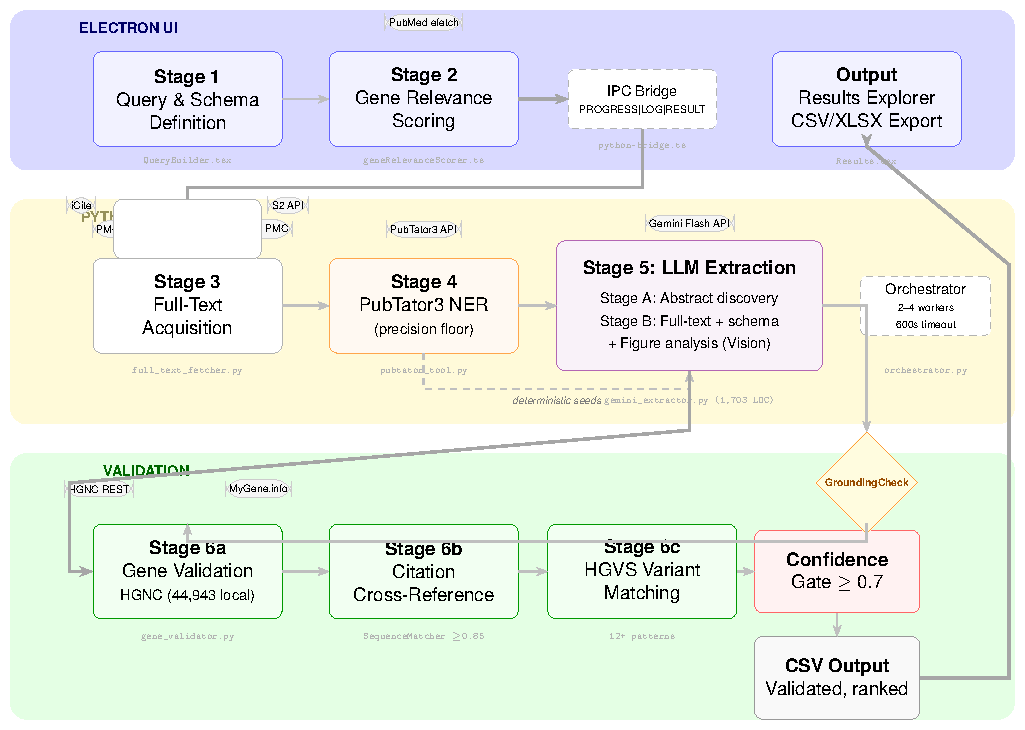
\includegraphics[width=0.94\textwidth]{figures/pipeline_tikz.pdf}
    \caption{ResearchShop system architecture. The Electron UI layer (top) handles query input, gene relevance scoring, and results display. The Python pipeline (middle) executes open-access full-text reading, candidate discovery, Gemini detail extraction, and output writing in a multiprocessing worker pool. The validation framework (bottom) applies gene symbol verification, grounding, citation cross-referencing, and a strict confidence gate ($\geq$0.7) before output.}
    \label{fig:architecture}
\end{figure*}

\subsection{Hybrid NER-LLM Architecture}

A key design decision is the \emph{hybrid} approach combining two complementary extraction strategies:

\begin{itemize}[itemsep=2pt]
    \item \textbf{PubTator3 (NER):} High precision, lower recall. Trained on annotated biomedical literature; genes it identifies are typically valid biomedical entities. Cannot extract contextual information (disease associations, functional impact, statistical evidence).
    \item \textbf{Gemini 2.5 Flash Lite (LLM, default):} High recall, lower precision. Extracts contextual relationships, statistical evidence, and citations. Prone to hallucination---generating gene symbols from training data that do not appear in the source paper.
\end{itemize}

The combination operates as follows: PubTator provides the precision floor (safety net), deterministic HGNC scanning adds source-grounded recall, and Gemini full-text candidate discovery extends coverage before schema-specific detail extraction. PubTator and deterministic candidates are injected as source-derived seeds into the LLM prompt, reducing the hallucination surface. A grounding check then verifies that \emph{every} LLM-extracted gene appears as text in the fetched paper, using the canonical symbol, HGNC aliases, biomedical mention bridges such as IFN-gamma to \textit{IFNG}, and the raw label the LLM used.

\subsection{Schema-Driven Extraction}

Users define custom output columns as natural-language descriptions. For example, researchers might specify:

\begin{itemize}[itemsep=1pt]
    \item \textbf{Key Finding}: Main research finding for this gene
    \item \textbf{Statistical Evidence}: p-values, odds ratios, confidence intervals
    \item \textbf{Functional Impact}: Effect on protein function or pathway
\end{itemize}

The pipeline dynamically constructs LLM prompts incorporating these column definitions, enabling researchers to customise extraction for different contexts (pharmacogenomics, rare diseases, cancer genomics) without code modifications. For each extracted value, the LLM is required to provide a verbatim citation from the source text.

\subsection{Desktop Application}
\label{subsec:desktop}

The application is packaged with electron-builder. The current public release provides a macOS \texttt{.dmg}; Windows \texttt{.exe} and Linux \texttt{.AppImage}/\texttt{.deb} targets are supported by the build configuration and remain part of release validation. On first launch, the application automatically creates a Python virtual environment and installs pipeline dependencies.

The GUI provides:
\begin{itemize}[itemsep=1pt]
    \item \textbf{Onboarding wizard:} API key validation, output directory selection, research-use disclaimer.
    \item \textbf{Query builder:} PubMed search with relevance scoring and paper selection.
    \item \textbf{Live pipeline monitor:} Real-time progress, per-stage breakdown, Gemini API usage tracking, and technical logs for debugging failed runs.
    \item \textbf{Results explorer:} Sortable table with confidence badges (CORROBORATED, SUPPORTED, LIMITED EVIDENCE, NEEDS REVIEW), plain-language confidence explanations, evidence/provenance fields, and CSV/XLSX export.
\end{itemize}

Security measures include OS-keychain-backed API key encryption (via Electron \texttt{safeStorage}), Content Security Policy headers, IPC path traversal validation, sandboxed renderer, and PMID input sanitisation.

\FloatBarrier
\subsection{Validation Framework}
\label{subsec:validation}

The validation framework treats the LLM output as an untrusted draft. Gemini is allowed to propose structured rows and fill user-defined fields, but the pipeline decides whether a row is exportable by re-checking the row against source text, controlled vocabularies, and deterministic pattern matchers. The checks are deliberately simple and auditable: each accepted or rejected row can be traced to explicit evidence rather than to a second opaque model decision.

\subsubsection{LLM Output Validation Heuristics}

For each paper, validation begins with a constrained candidate set assembled from PubTator3 entities, deterministic HGNC symbol and alias scanning, and Gemini candidate discovery. The detail-extraction prompt receives this candidate context and is instructed to provide citations for every extracted claim. The returned rows are then processed by the following deterministic heuristics:

\begin{enumerate}[itemsep=2pt]
    \item \textbf{Identifier normalisation.} The reported gene string is mapped to an HGNC-approved symbol when possible. Previous symbols and aliases are retained as provenance, but the exported gene field uses the canonical symbol.
    \item \textbf{Source presence.} The canonical symbol, any HGNC alias, or the raw mention supplied by the LLM must occur in the fetched article text. This rejects real but off-topic genes that the model may know from pre-training but that are absent from the paper.
    \item \textbf{Citation anchoring.} The citation or evidence quote supplied by the LLM is matched back to the article using normalized dense sequence matching. Rows with citation-bearing fields are removed from the primary export when none of the supplied citations can be grounded.
    \item \textbf{Local gene context.} A matched citation must be near the relevant gene mention, not merely somewhere in the same article. This reduces errors where a generic disease or pathway sentence is attached to the wrong gene.
    \item \textbf{Numerical preservation.} Numeric tokens in the LLM citation, such as p-values, odds ratios, cohort sizes, or variant positions, must be present in the matched source passage. This catches a common failure mode where an LLM preserves the qualitative claim but invents or alters the quantitative detail.
    \item \textbf{Variant sanity check.} Variant-like strings are tested against HGVS-oriented regular-expression patterns. Non-matching variants can remain visible as review metadata, but they are not treated as validated HGVS evidence.
    \item \textbf{Hard gates before export.} Identifier resolution, source presence, and row-level citation anchoring are treated as required gates for the primary CSV. The citation matcher also enforces local gene context and numeric preservation inside the citation decision. A row that fails a required gate is retained only in review or drop-debug artifacts; it cannot pass solely because its gene symbol is HGNC-valid.
    \item \textbf{Confidence label and audit trail.} Rows that pass the required gates receive a confidence score and a plain-language label. Rows below the configured threshold are omitted from the primary CSV and recorded with the failed check, allowing users to inspect false negatives.
\end{enumerate}

These heuristics are not presented as a substitute for expert curation. Their purpose is to make the LLM's contribution bounded: the model may summarize and structure evidence, but exported associations must be tied back to text that ResearchShop can locate in the paper.

\begin{table*}[t]
\centering
\small
\setlength{\tabcolsep}{5pt}
\renewcommand{\arraystretch}{1.08}
\begin{tabularx}{\textwidth}{>{\raggedright\arraybackslash}p{2.7cm} >{\raggedright\arraybackslash}X >{\raggedright\arraybackslash}p{3.5cm} >{\raggedright\arraybackslash}p{3.0cm}}
\toprule
\textbf{Check} & \textbf{Decision rule} & \textbf{Failure addressed} & \textbf{Primary output action} \\
\midrule
HGNC normalization & Map the LLM gene string to an approved symbol using the local HGNC snapshot, aliases, previous symbols, HGNC REST, or MyGene.info fallback. & Invalid symbols, obsolete labels, ambiguous aliases. & Required gate; unresolved symbols are excluded from the primary CSV. \\
Source grounding & Require the canonical symbol, an alias, or the raw LLM mention to occur in fetched article text. & Real but off-paper genes introduced from model prior knowledge. & Required gate; failures go to review/drop artifacts. \\
Citation anchoring & Match the LLM evidence quote to article text after normalization using \texttt{SequenceMatcher} threshold $\geq 0.85$. & Fabricated or unlocatable citations. & Required row-level gate when citation fields are present; at least one supplied citation must ground. \\
Local gene context & Require the gene or alias near the matched evidence span. & Correct source sentence attached to the wrong gene. & Enforced inside citation validation. \\
Numeric preservation & Require source matches for p-values, odds ratios, cohort sizes, positions, and other numeric tokens. & Altered statistics or invented quantitative detail. & Enforced inside citation validation when numeric claims are present. \\
Variant validation & Match variant-like strings against HGVS-oriented protein, coding, genomic, splice, indel, copy-number, and cytogenetic patterns. & Malformed variants or unsupported nomenclature. & Variant confidence only; unvalidated variants remain review metadata. \\
Confidence gate & After required gates pass, export rows only when $C_{\mathrm{total}} \geq 0.7$. & Weakly supported associations. & Below-threshold rows are omitted and audited. \\
\bottomrule
\end{tabularx}
\caption{Deterministic decision model used to validate LLM-generated extraction rows before export.}
\label{tab:llm_validation_decisions}
\end{table*}

The validation framework then applies four implementation layers, each targeting different error types:

\subsubsection{Gene Symbol Validation}
Every extracted gene is verified against authoritative databases in priority order:
\begin{enumerate}[itemsep=1pt]
    \item \textbf{Local HGNC database:} A bundled snapshot of 44,943 HGNC entries (19,297 protein-coding) enables offline lookups of official symbols, aliases, and previous symbols.
    \item \textbf{HGNC REST API:} Fallback for genes not found locally (e.g., recently approved symbols).
    \item \textbf{MyGene.info:} Second fallback providing additional alias coverage.
    \item \textbf{Fuzzy matching:} Suggests corrections for near-misses (e.g., ``BRAC1'' $\to$ ``BRCA1'').
\end{enumerate}

Biotype information is retained as metadata so researchers can distinguish protein-coding genes, non-coding RNA genes, pseudogenes, and other HGNC locus classes during review. The current release does not reject valid HGNC symbols solely because they are non-protein-coding; this avoids false negatives in RNA-seq, regulatory RNA, and immunogenomics workflows.

\subsubsection{Grounding Check}
The grounding check verifies that each candidate gene symbol appears as text in the fetched paper. This prevents ``contextual hallucinations'' where the LLM mentions real genes from its training data that are not discussed in the paper. The check searches for the canonical symbol, all HGNC aliases, and the raw label the LLM used (e.g., ``BNP'' for NPPB).

\subsubsection{Variant Pattern Matching}
Extracted variants are validated against 12+ HGVS nomenclature patterns~\cite{denDunnen2016hgvs}: protein substitution (\texttt{p.Arg175His}), coding variants (\texttt{c.1234A>G}), genomic variants (\texttt{g.123456A>T}), frameshifts, splice sites, indels, copy number states, translocations, and cytogenetic notation. Both three-letter and single-letter amino acid codes are recognised.

\subsubsection{Citation Cross-Referencing}
For each LLM-provided citation, the system verifies its existence in the paper text using dense sequence matching (\texttt{difflib.SequenceMatcher}, threshold~$\geq$0.85). Additional checks include:
\begin{itemize}[itemsep=1pt]
    \item \textbf{Numerical consistency:} All numbers in the citation must exist in the matched paragraph.
    \item \textbf{Gene context:} The gene symbol or an alias must appear within $\pm$1,500 characters of the citation match.
    \item \textbf{Encoding normalisation:} Unicode slash variants, LaTeX Greek commands, and ASCII prefixes are normalised symmetrically on both sides before matching.
\end{itemize}

\subsubsection{Confidence Scoring and Strict Gate}
Primary CSV export is a two-step decision. First, required validation gates must pass: HGNC normalization, source grounding, and row-level citation anchoring when citation fields are present. The citation validator itself rejects matches that lack local gene context or preserve inconsistent numeric claims. Second, rows that pass these gates receive a confidence score:
\begin{equation}
C_{\mathrm{total}} = C_g + C_v
\label{eq:confidence}
\end{equation}
where $C_g = 0.7$ if the gene passes HGNC validation (1.0 for gene-only associations) and $C_v = 0.3$ if the variant passes HGVS pattern matching. The strict validation gate (\texttt{FINAL\_VALIDATION\_MIN\_CONFIDENCE=0.7}) filters associations below this threshold from the output CSV. Therefore a row with a valid HGNC symbol but failed source grounding or no grounded citation among its supplied citation fields is not exported merely because $C_g$ reaches 0.7; the hard gates must pass first. This conservative threshold favours source-grounded precision over broader recall in the default research-triage workflow.
